\documentclass[11pt,a4paper]{article}

% ---------------------------------------------------------------------------
% Packages
% ---------------------------------------------------------------------------
\usepackage[margin=1in]{geometry}
\usepackage{lmodern}
\usepackage[T1]{fontenc}
\usepackage[utf8]{inputenc}
\usepackage{microtype}
\setlength{\headheight}{22pt}
\addtolength{\topmargin}{-10pt}
\usepackage{amsmath,amssymb,amsthm}
\usepackage{mathtools}
\usepackage{enumitem}
\usepackage{booktabs}
\usepackage{array}
\usepackage{xcolor}
\usepackage{hyperref}
\usepackage[nameinlink,noabbrev]{cleveref}
\usepackage{listings}
\usepackage{caption}
\usepackage{setspace}
\usepackage{titlesec}
\usepackage{fancyhdr}
\usepackage{tikz}
\usetikzlibrary{arrows.meta,positioning,calc}

% ---------------------------------------------------------------------------
% Colors & links
% ---------------------------------------------------------------------------
\definecolor{ink}{HTML}{1A1A1A}
\definecolor{accent}{HTML}{0B3D5C}
\definecolor{rulegray}{HTML}{C8CDD2}
\definecolor{codebg}{HTML}{F6F8FA}
\definecolor{codekw}{HTML}{0B3D5C}
\definecolor{codestr}{HTML}{8A4B08}
\definecolor{codecom}{HTML}{5B6B73}

\hypersetup{
  colorlinks=true,
  linkcolor=accent,
  citecolor=accent,
  urlcolor=accent,
  pdftitle={On the Uniqueness of the Even Prime},
  pdfauthor={Machine-Checked Notes},
  pdfsubject={Elementary number theory; interactive theorem proving}
}

% ---------------------------------------------------------------------------
% Typography
% ---------------------------------------------------------------------------
\onehalfspacing
\setlength{\parskip}{0.35em}
\setlength{\parindent}{1.2em}

\titleformat{\section}
  {\large\bfseries\color{accent}}{\thesection}{0.75em}{}
  [{\color{rulegray}\titlerule[0.4pt]}]
\titleformat{\subsection}
  {\normalsize\bfseries\color{ink}}{\thesubsection}{0.75em}{}
\titleformat{\subsubsection}
  {\normalsize\itshape\color{ink}}{\thesubsubsection}{0.75em}{}

\titlespacing*{\section}{0pt}{1.6em}{0.8em}
\titlespacing*{\subsection}{0pt}{1.2em}{0.5em}

% ---------------------------------------------------------------------------
% Header / footer
% ---------------------------------------------------------------------------
\pagestyle{fancy}
\fancyhf{}
\fancyhead[L]{\small\color{accent}On the Uniqueness of the Even Prime}
\fancyhead[R]{\small\color{ink}\thepage}
\renewcommand{\headrulewidth}{0.3pt}
\renewcommand{\headrule}{\hbox to\headwidth{\color{rulegray}\leaders\hrule height \headrulewidth\hfill}}
\fancypagestyle{plain}{%
  \fancyhf{}%
  \fancyfoot[C]{\small\color{ink}\thepage}%
  \renewcommand{\headrulewidth}{0pt}%
}

% ---------------------------------------------------------------------------
% Theorem environments
% ---------------------------------------------------------------------------
\theoremstyle{plain}
\newtheorem{theorem}{Theorem}[section]
\newtheorem{lemma}[theorem]{Lemma}
\newtheorem{proposition}[theorem]{Proposition}
\newtheorem{corollary}[theorem]{Corollary}

\theoremstyle{definition}
\newtheorem{definition}[theorem]{Definition}
\newtheorem{remark}[theorem]{Remark}

\theoremstyle{remark}
\newtheorem*{claim}{Claim}

% ---------------------------------------------------------------------------
% Listings (Lean fragments)
% ---------------------------------------------------------------------------
\lstdefinelanguage{Lean}{
  morekeywords={theorem,lemma,def,example,namespace,end,import,
    by,exact,intro,have,obtain,refine,cases,constructor,
    fun,forall,exists,Prop,Nat,True,False,classical,
    if,then,else,match,with,structure,inductive,where},
  sensitive=true,
  morecomment=[l]{--},
  morecomment=[s]{/-}{-/},
  morestring=[b]"
}

\lstset{
  language=Lean,
  basicstyle=\ttfamily\small,
  backgroundcolor=\color{codebg},
  keywordstyle=\bfseries\color{codekw},
  commentstyle=\itshape\color{codecom},
  stringstyle=\color{codestr},
  frame=single,
  rulecolor=\color{rulegray},
  framesep=6pt,
  xleftmargin=4pt,
  xrightmargin=4pt,
  breaklines=true,
  columns=fullflexible,
  keepspaces=true,
  showstringspaces=false,
  tabsize=2,
  aboveskip=0.9em,
  belowskip=0.9em
}

\captionsetup{font=small,labelfont={bf,color=accent}}

% ---------------------------------------------------------------------------
% Helpers
% ---------------------------------------------------------------------------
\newcommand{\N}{\mathbb{N}}
\newcommand{\Lean}{\textsc{Lean}}
\DeclareMathOperator{\IsPrime}{IsPrime}
\DeclareMathOperator{\IsEven}{IsEven}

% ---------------------------------------------------------------------------
\begin{document}

% ============================== Title page ==============================
\begin{titlepage}
\thispagestyle{empty}
\centering
\vspace*{1.8cm}

{\color{accent}\rule{0.55\textwidth}{0.6pt}}\\[0.9em]
{\LARGE\bfseries\color{accent} On the Uniqueness of the Even Prime}\\[0.55em]
{\large Five Elementary Proofs, a Two-Sided Strengthening,\\
and a Machine-Checked Formalization}\\[0.9em]
{\color{accent}\rule{0.55\textwidth}{0.6pt}}

\vspace{1.6cm}

{\large A short note in elementary number theory\\
with a companion development in \Lean{}~4}

\vspace{1.4cm}

\begin{tikzpicture}[
  box/.style={draw=accent, rounded corners=2pt, align=center,
              inner sep=7pt, font=\small, text=ink, fill=codebg},
  arr/.style={-{Latex}, accent, thick}
]
\node[box] (below) {No even prime\\$n < 2$};
\node[box, right=1.5cm of below] (above) {No even prime\\$n > 2$};
\node[box, below=1.1cm of $(below)!0.5!(above)$] (two) {$2$ is an even prime};
\node[box, below=1.1cm of two, fill=white, line width=0.9pt] (grand)
  {Unique even prime is $2$};
\draw[arr] (below) -- (grand);
\draw[arr] (above) -- (grand);
\draw[arr] (two) -- (grand);
\end{tikzpicture}

\vfill

{\small\color{ink}
Compiled from a \Lean{}~4 formalization (stdlib only, no Mathlib).\\
All theorems stated below have been checked by the \Lean{} kernel.}

\vspace{1.2cm}
{\small\color{codecom}\today}
\end{titlepage}
\setcounter{page}{1}
\pagenumbering{arabic}

% ============================== Abstract ==============================
\begin{abstract}
\noindent
We give a careful elementary treatment of the classical fact that
\emph{$2$ is the unique even prime number}. Five distinct proofs that
there is no even prime greater than~$2$ are presented, together with the
complementary observation that there is no even prime less than~$2$.
From this expansive, two-sided picture we recover the grand uniqueness
statement. We then discuss the specification gap inherent in interactive
theorem proving---the distinction between verifying a formal derivation
and validating that a formal statement matches an informal claim---and
record how a companion \Lean{}~4 development closes as much of that gap
as is possible inside the prover.
\end{abstract}

\tableofcontents
\vspace{0.6em}
{\color{rulegray}\hrule height 0.4pt}
\vspace{1.2em}

% ============================== 1 ==============================
\section{Introduction}
\label{sec:intro}

Among the first nontrivial observations one meets in elementary number
theory is that evenness and primality interact in a very rigid way:
once a natural number is divisible by~$2$ and strictly larger than~$2$,
it cannot be prime. Consequently the only even prime is~$2$ itself.

The argument is short enough to fit in a sentence, yet rich enough to
illustrate several standard proof patterns---direct reasoning from the
definition, contraposition, contradiction, an appeal to the uniqueness
of prime divisors, and a least-counterexample (well-ordering) argument.
The same fact also admits a clean ``two-sided'' packaging: there are no
even primes below~$2$ and none above~$2$, while~$2$ itself is an even
prime. Trichotomy on~$\N$ then yields uniqueness at a stroke.

The purpose of this note is twofold. First, we write the mathematics
cleanly, with explicit definitions and several independent proofs.
Second, we record how the same material was formalized in \Lean{}~4 and
how one can increase confidence that the formal theorems match the
intended informal claim.

% ============================== 2 ==============================
\section{Preliminaries}
\label{sec:prelim}

Throughout, $\N$ denotes the nonnegative integers
$\{0,1,2,\ldots\}$. Divisibility is written $d \mid n$.

\begin{definition}[Prime]
\label{def:prime}
A natural number $n$ is \emph{prime} if $n > 1$ and every positive
divisor of~$n$ is either~$1$ or~$n$. In symbols,
\[
  \IsPrime(n)
  \;\stackrel{\mathrm{def}}{\Longleftrightarrow}\;
  n > 1
  \;\land\;
  \bigl(\forall\, d \in \N,\ d \mid n \Rightarrow d=1 \lor d=n\bigr).
\]
\end{definition}

\begin{definition}[Even]
\label{def:even}
A natural number $n$ is \emph{even} if $2 \mid n$. In symbols,
\[
  \IsEven(n)
  \;\stackrel{\mathrm{def}}{\Longleftrightarrow}\;
  2 \mid n.
\]
\end{definition}

\begin{remark}
These are the usual textbook characterizations. Equivalently,
$\IsEven(n)$ if and only if $n \bmod 2 = 0$, and $\IsPrime(n)$ if and
only if $n>1$ and $n$ has no divisor~$d$ with $1 < d < n$. Both
equivalences are routine and were checked in the companion
formalization.
\end{remark}

\begin{lemma}[Two is an even prime]
\label{lem:two}
We have $\IsPrime(2)$ and $\IsEven(2)$.
\end{lemma}

\begin{proof}
Evenness is immediate: $2 = 2\cdot 1$. For primality, the only
positive divisors of~$2$ are~$1$ and~$2$, which one verifies by noting
that any positive divisor~$d$ satisfies $d \le 2$.
\end{proof}

% ============================== 3 ==============================
\section{No even prime greater than two}
\label{sec:above}

We first prove the ``upper'' half of the story.

\begin{theorem}
\label{thm:above}
If $n > 2$ and $\IsEven(n)$, then $\neg\,\IsPrime(n)$.
Equivalently: every even natural number greater than~$2$ is composite.
\end{theorem}

We give five proofs. Each establishes the same mathematical content by
a different organizing idea; all five have been checked independently
in \Lean{}.

\subsection{Proof~A: Direct from the definition}
\label{sec:proofA}

\begin{proof}[Proof~A]
Let $p$ be prime and even. Then $2 \mid p$. By~\Cref{def:prime} every
positive divisor of~$p$ equals~$1$ or~$p$, so $2=1$ or $2=p$. The first
alternative is absurd, hence $p=2$. In particular, no even prime can
exceed~$2$.
\end{proof}

\subsection{Proof~B: Contrapositive}
\label{sec:proofB}

\begin{proof}[Proof~B]
Let $n>2$ be even, and write $n = 2k$. Then $k > 1$ (since $n>2$) and
$k < n$ (since $k = n/2$). Thus $k$ is a positive divisor of~$n$
strictly between~$1$ and~$n$, so $n$ is not prime.
\end{proof}

\subsection{Proof~C: Contradiction}
\label{sec:proofC}

\begin{proof}[Proof~C]
Suppose $p$ is an even prime with $p \neq 2$. Then $2 \mid p$, and
primality forces $2=1$ or $2=p$. Both are impossible under the standing
assumptions, a contradiction.
\end{proof}

\subsection{Proof~D: Prime divisibility}
\label{sec:proofD}

\begin{lemma}
\label{lem:prime-dvd-prime}
If $p$ and $q$ are prime and $p \mid q$, then $p=q$.
\end{lemma}

\begin{proof}
By primality of~$q$, the divisor~$p$ equals~$1$ or~$q$. But $p>1$, so
$p=q$.
\end{proof}

\begin{proof}[Proof~D]
Let $p$ be an even prime. Then $2 \mid p$. Since~$2$ is itself prime
(\Cref{lem:two}), \Cref{lem:prime-dvd-prime} yields $2=p$.
\end{proof}

\subsection{Proof~E: Least counterexample}
\label{sec:proofE}

\begin{lemma}[Well-ordering form]
\label{lem:least}
If a predicate $P$ on~$\N$ holds for some natural number, then there
exists a least such number: some $m$ with $P(m)$ and
$\neg P(k)$ for all $k<m$.
\end{lemma}

\begin{proof}[Proof~E]
Suppose there exists an even prime greater than~$2$, and let~$m$ be a
least such number (\Cref{lem:least}). Then $m$ is even and $m>2$, so
the argument of Proof~B shows that~$m$ is composite---contradicting
the choice of~$m$. Hence no even prime greater than~$2$ exists.
\end{proof}

\begin{remark}
For this particular theorem the appeal to minimality is logically
redundant: \emph{every} even integer greater than~$2$ is immediately
composite. The least-counterexample packaging is included because it
is a standard pattern, and because the well-ordering lemma itself is
of independent interest.
\end{remark}

\begin{corollary}
\label{cor:above-unique}
If $\IsPrime(p)$ and $\IsEven(p)$, then $p=2$.
\end{corollary}

\begin{proof}
If $p>2$, \Cref{thm:above} forbids primality. Since every prime
satisfies $p>1$, the remaining possibility compatible with evenness is
$p=2$.
\end{proof}

% ============================== 4 ==============================
\section{No even prime less than two}
\label{sec:below}

The complementary ``lower'' half is even shorter, and in fact does not
use evenness at all.

\begin{theorem}
\label{thm:below}
If $n < 2$, then $\neg\,\IsPrime(n)$.
In particular, there is no even prime less than~$2$.
\end{theorem}

\begin{proof}
By~\Cref{def:prime}, every prime satisfies $n>1$. On~$\N$ the condition
$n<2$ is incompatible with $n>1$. Explicitly, the only candidates are
$n=0$ and $n=1$, neither of which is greater than~$1$.
\end{proof}

\begin{remark}
One may equally argue by exhaustion on $\{0,1\}$, or by quoting the
characterization ``$\IsPrime(n)\Rightarrow n>1$'' obtained from
auditing~\Cref{def:prime}. All of these variants appear in the
companion \Lean{} file.
\end{remark}

% ============================== 5 ==============================
\section{The grand uniqueness theorem}
\label{sec:grand}

We now assemble the two sides into a single expansive picture and
deduce uniqueness.

\begin{definition}[Expansive even-prime picture]
\label{def:expansive}
The \emph{expansive even-prime picture} is the conjunction of the
following four assertions:
\begin{enumerate}[label=(\alph*),leftmargin=2.2em]
  \item there is no even prime $n<2$;
  \item there is no even prime $n>2$;
  \item $\IsPrime(2)$;
  \item $\IsEven(2)$.
\end{enumerate}
\end{definition}

\begin{theorem}[Grand uniqueness]
\label{thm:grand}
The following are equivalent:
\begin{enumerate}[label=(\roman*),leftmargin=2.2em]
  \item the expansive even-prime picture holds;
  \item $\forall\, p\in\N,\ \IsPrime(p) \rightarrow \IsEven(p)
        \rightarrow p=2$;
  \item $2$ is an even prime, and it is the only one;
  \item $\neg\exists\, p\in\N$ such that
        $\IsPrime(p)\land\IsEven(p)\land p\neq 2$.
\end{enumerate}
In particular, there is no even prime aside from~$2$.
\end{theorem}

\begin{proof}
The implications among (ii)--(iv) are pure propositional rearrangements;
we focus on the passage through the expansive picture.

\medskip
\noindent\textit{(i)\,$\Rightarrow$\,(ii).}
Assume the expansive picture, and let $p$ be an even prime. By
trichotomy on~$\N$, exactly one of $p<2$, $p=2$, or $p>2$ holds.
The first case is ruled out by~(a), the third by~(b), and therefore
$p=2$.

\medskip
\noindent\textit{(ii)\,$\Rightarrow$\,(i).}
Clauses~(c) and~(d) are~\Cref{lem:two}. Clause~(a)
is~\Cref{thm:below}. For~(b): if $n>2$ is even and prime,
then~(ii) forces $n=2$, contradicting $n>2$.

\medskip
\noindent\textit{(ii)\,$\Leftrightarrow$\,(iii)\,$\Leftrightarrow$\,(iv).}
Immediate from~\Cref{lem:two} and first-order logic.
\end{proof}

\begin{corollary}
\label{cor:unique}
The unique even prime natural number is~$2$.
\end{corollary}

% ============================== 6 ==============================
\section{On matching statements to proofs}
\label{sec:spec}

Interactive theorem provers such as \Lean{} check a judgment of the
form $\Gamma \vdash t : T$: under context~$\Gamma$, the term~$t$ has
type~$T$. When $T$ is a proposition, this is a formal proof of~$T$.
What the kernel \emph{cannot} check is that $T$ correctly renders an
English sentence. This is the classical
\emph{specification gap} between verification and validation
\cite{deMillo1979,Asperti2007}.

\subsection{What remains trusted}

After formalization, a human must still accept a small
\emph{reading surface}. In our development that surface is essentially
\begin{lstlisting}
def TargetClaim : Prop :=
  forall p : Nat, IsPrime p -> IsEven p -> p = 2
\end{lstlisting}
together with the definitions of $\IsPrime$ and $\IsEven$
from~\Cref{sec:prelim}. Everything else is derived.

\subsection{What can be machine-checked}

Inside the prover one can still compress that trust surface
substantially:
\begin{enumerate}[leftmargin=1.4em]
  \item \textbf{Independent restatements.}
        Formalize the intended claim in several equivalent ways
        (uniqueness; nonexistence of any other even prime; compositeness
        of all even $n>2$) without referring to the proof theorems, then
        prove the restatements equivalent.
  \item \textbf{Proof--claim alignment.}
        Show that each concrete proof theorem inhabits exactly the
        target proposition (and conversely).
  \item \textbf{Definition audits.}
        Prove $\IsEven(n)\leftrightarrow (n\bmod 2=0)$ and the
        ``no proper divisor'' characterization of primality, so that a
        silently wrong encoding is unlikely to survive.
  \item \textbf{Anti-triviality.}
        Exhibit an even prime, an odd prime, and an even composite; show
        that the false claim ``every even prime equals~$3$'' is refuted.
        These tests catch vacuous or collapsed definitions.
\end{enumerate}

In the companion development these steps are packaged as a single
\emph{specification certificate}, which the \Lean{} kernel accepts.

% ============================== 7 ==============================
\section{The Lean formalization}
\label{sec:lean}

The accompanying \Lean{}~4 project uses only the standard library (no
Mathlib), so that a bare toolchain suffices to check it. The module
layout mirrors the mathematics of this note:

\begin{center}
\small
\begin{tabular}{@{}ll@{}}
\toprule
\textbf{Module} & \textbf{Contents} \\
\midrule
\texttt{EvenPrime/Prime.lean}
  & $\IsPrime$, $\IsEven$, \Cref{lem:two}, \Cref{lem:prime-dvd-prime} \\
\texttt{EvenPrime/Proofs.lean}
  & Five proofs of~\Cref{thm:above}/\Cref{cor:above-unique} \\
\texttt{EvenPrime/BelowTwo.lean}
  & \Cref{thm:below} and variants \\
\texttt{EvenPrime/Grand.lean}
  & Expansive picture and~\Cref{thm:grand} \\
\texttt{EvenPrime/Spec.lean}
  & Specification certificate (\Cref{sec:spec}) \\
\texttt{EvenPrime/Tests.lean}
  & Concrete computational checks \\
\bottomrule
\end{tabular}
\end{center}

\noindent
A representative fragment of the grand theorem reads as follows.

\begin{lstlisting}
theorem no_even_prime_aside_from_two_of_expansive
    (H : ExpansiveEvenPrimePicture) :
    NoEvenPrimeAsideFromTwo := by
  obtain <hBelow, hAbove, _, _> := H
  intro p hp he
  by_cases hlt : p < 2
  . exact False.elim (hBelow p hlt he hp)
  . by_cases hgt : p > 2
    . exact False.elim (hAbove p hgt he hp)
    . omega
\end{lstlisting}

Concrete regression tests confirm, among other things, that
$2$ is even and prime while $4,6,8,100$ are even and not prime, and
that odd primes such as $3,5,7$ remain prime under the formal
definition.

% ============================== 8 ==============================
\section{Conclusion}
\label{sec:concl}

The uniqueness of the even prime is elementary, but it is also a tidy
microcosm of mathematical practice: a crisp definition, several genuine
proof ideas, a two-sided strengthening that makes uniqueness inevitable
by trichotomy, and---once one formalizes---a reminder that the last inch
of trust is always a human reading of a top-level statement. Within that
discipline, the grand claim stands:

\begin{quote}
\centering\itshape
There is no even prime natural number aside from~$2$.
\end{quote}

% ============================== Appendix ==============================
\appendix
\section{Logical relationships at a glance}
\label{app:diagram}

The following diagram summarizes the equivalences checked in the
formalization. Solid arrows are the constructive implications used in
the grand proof; dashed edges indicate propositional equivalences.

\begin{center}
\begin{tikzpicture}[
  every node/.style={font=\small},
  box/.style={draw=accent, rounded corners=2pt, align=center,
              inner sep=6pt, text=ink, fill=white},
  arr/.style={-{Latex}, accent, thick},
  eq/.style={accent, dashed, thick}
]
\node[box] (below) {No even prime $<2$};
\node[box, right=2.2cm of below] (above) {No even prime $>2$};
\node[box, below=1.0cm of $(below)!0.5!(above)$] (wit) {$2$ even \& prime};
\node[box, below=1.0cm of wit, line width=0.9pt] (grand)
  {$\forall p,\;\mathrm{prime}\land\mathrm{even}\Rightarrow p=2$};
\node[box, below left=1.1cm and -0.2cm of grand] (uniq)
  {Unique even prime is $2$};
\node[box, below right=1.1cm and -0.2cm of grand] (neg)
  {$\neg\exists\,p\neq 2$ even prime};

\draw[arr] (below) -- (grand);
\draw[arr] (above) -- (grand);
\draw[arr] (wit) -- (grand);
\draw[eq] (grand) -- (uniq);
\draw[eq] (grand) -- (neg);
\end{tikzpicture}
\end{center}

\section{Checklist for the trusted reading surface}
\label{app:checklist}

A reader wishing to validate---rather than merely verify---the
formalization need only confirm the following.

\begin{enumerate}[leftmargin=1.4em]
  \item $\IsPrime$ and $\IsEven$ match~\Cref{def:prime,def:even}.
  \item The target proposition is
        $\forall p,\ \IsPrime(p)\rightarrow\IsEven(p)\rightarrow p=2$.
  \item The expansive picture used in the grand proof is exactly
        \Cref{def:expansive}.
  \item The kernel accepts the development (e.g.\ via
        \texttt{lake build}).
\end{enumerate}

% ============================== Bibliography ==============================
\begin{thebibliography}{9}
\bibitem{deMillo1979}
R.~A.~De~Millo, R.~J.~Lipton, and A.~J.~Perlis,
\textit{Social processes and proofs of theorems and programs},
Communications of the ACM \textbf{22} (1979), no.~5, 271--280.

\bibitem{Asperti2007}
A.~Asperti, H.~Geuvers, and R.~Natarajan,
\textit{Social processes, program verification and all that},
Mathematical Structures in Computer Science
\textbf{19} (2009), no.~5, 877--896.
\end{thebibliography}

\end{document}
